\chapter{Property of sandpile model}\label{ch:introduction3}

\section{Q7 Avalanche Distributions}

\textbf{Record the frequency with which avalanches have a specific number of topples, area, loss and length. What kind of distribution do you get for each? If possible, can you find a fit for the distribution? (E.g. for a Gaussian, find the mean and width of the distribution; for a power law, find the exponent.)}

Question 7 asks us to record the frequency with which avalanches have a specific number of topples, area, loss and length, and to determine what kind of distribution is obtained for
each quantity. In the Bak--Tang--Wiesenfeld model, an avalanche is produced after adding
one grain of sand to the lattice and then repeatedly toppling unstable sites until the system
returns to a stable configuration.

In this simulation, I used a \(50 \times 50\) lattice and ran the model for \(10^5\) grain additions. No transient cutoff was applied, so avalanches were recorded from the beginning of the simulation. The random seed was fixed at \(41\), and grains were added using a uniform random distribution over the lattice sites.
As discussed in Section~\ref{sec:vardef}, the avalanche variables are defined before analysing their distributions.

\subsection{Histogram Results}

The ordinary histograms are shown in Figure~\ref{fig:q7_histograms}. They are strongly
right-skewed. In all four cases, small avalanches occur very frequently, while large avalanches
are much rarer. This already suggests that the distributions are not Gaussian. A Gaussian
distribution would be concentrated around a typical scale, whereas these avalanche
distributions contain many small events together with some rare but much larger events.

\begin{figure}[htbp]
    \centering

    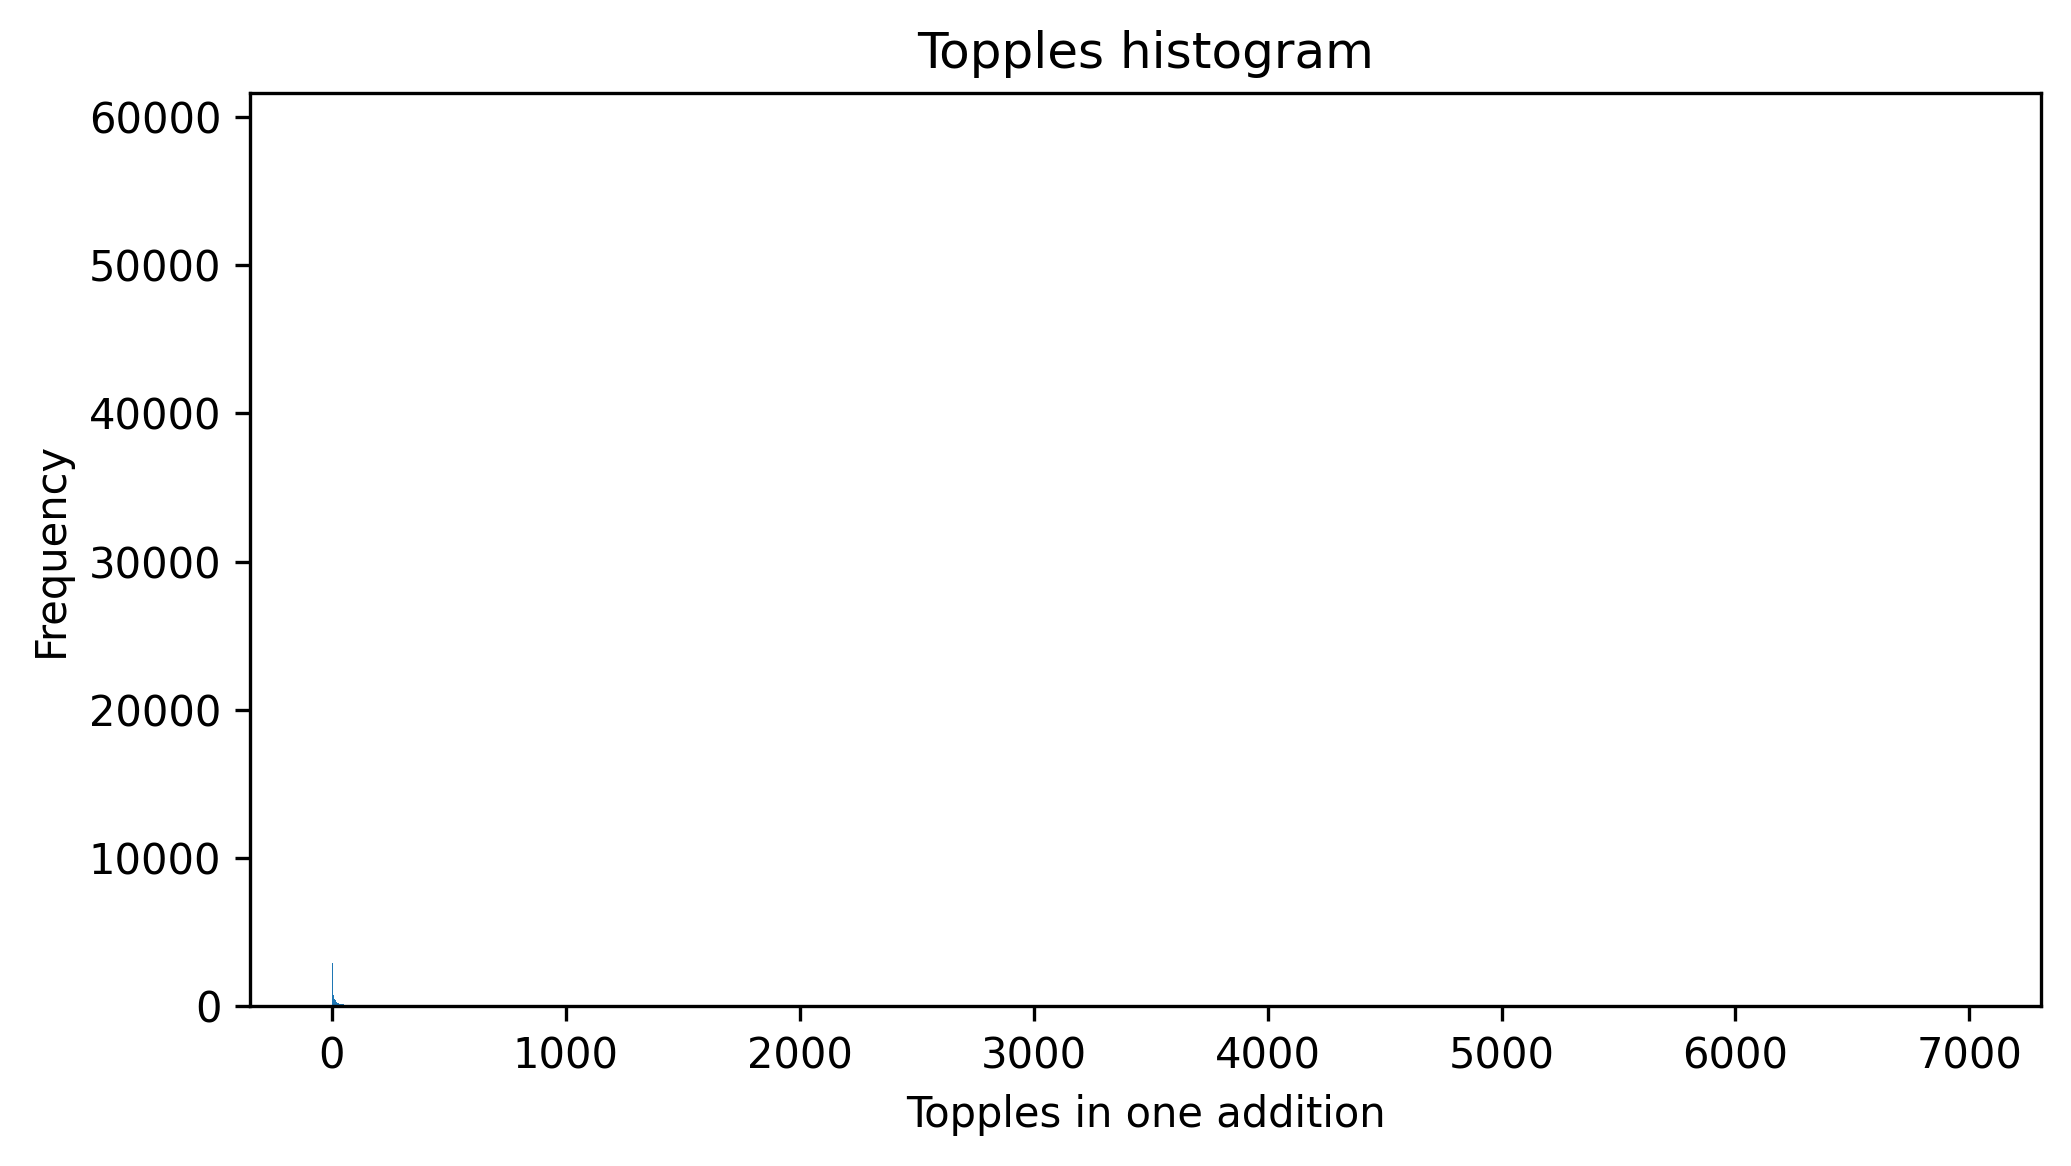
\includegraphics[width=0.45\textwidth]{figures/topple_histogram.png}
    \hfill
    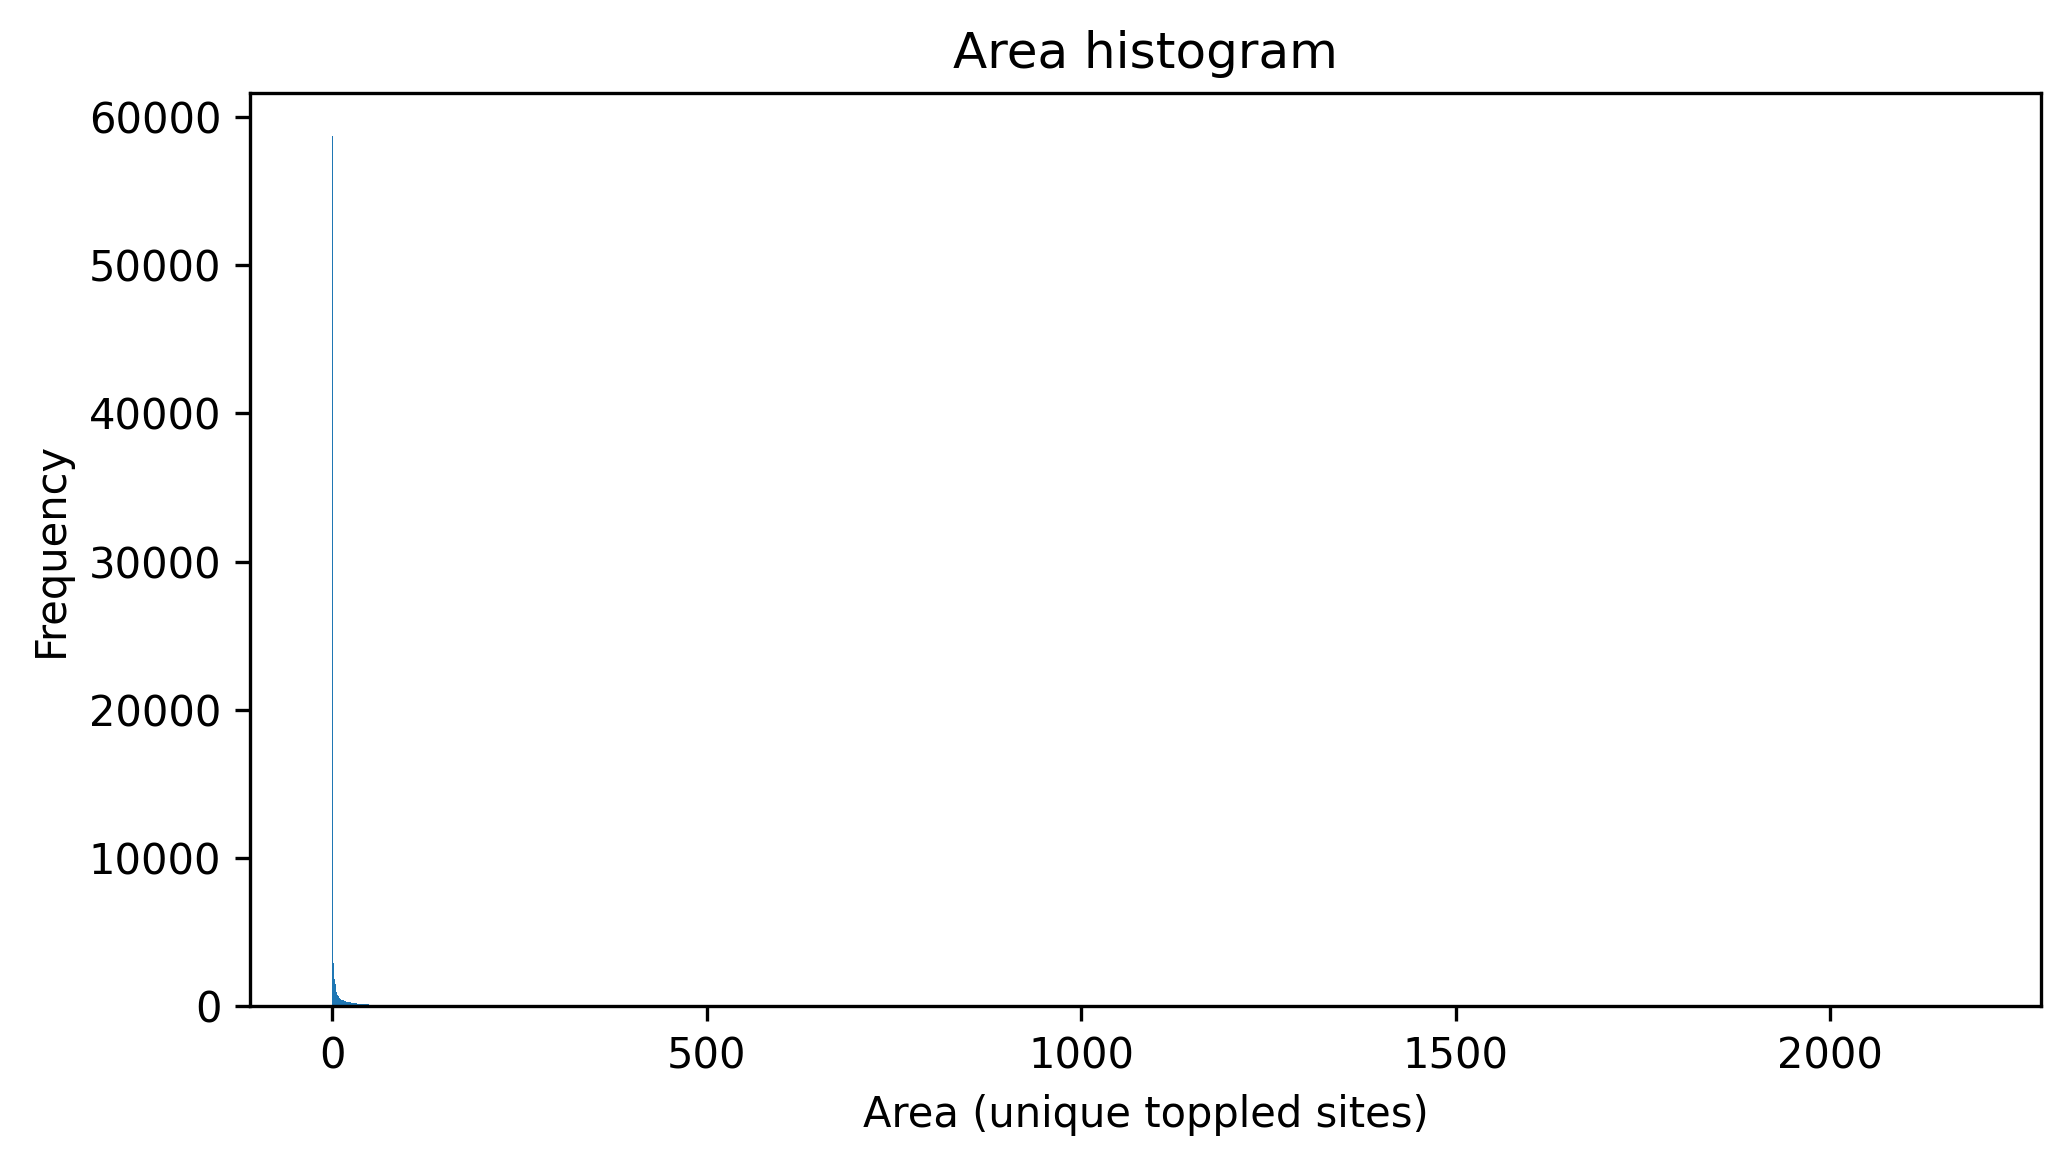
\includegraphics[width=0.45\textwidth]{figures/area_histogram.png}

    \vspace{0.4cm}

    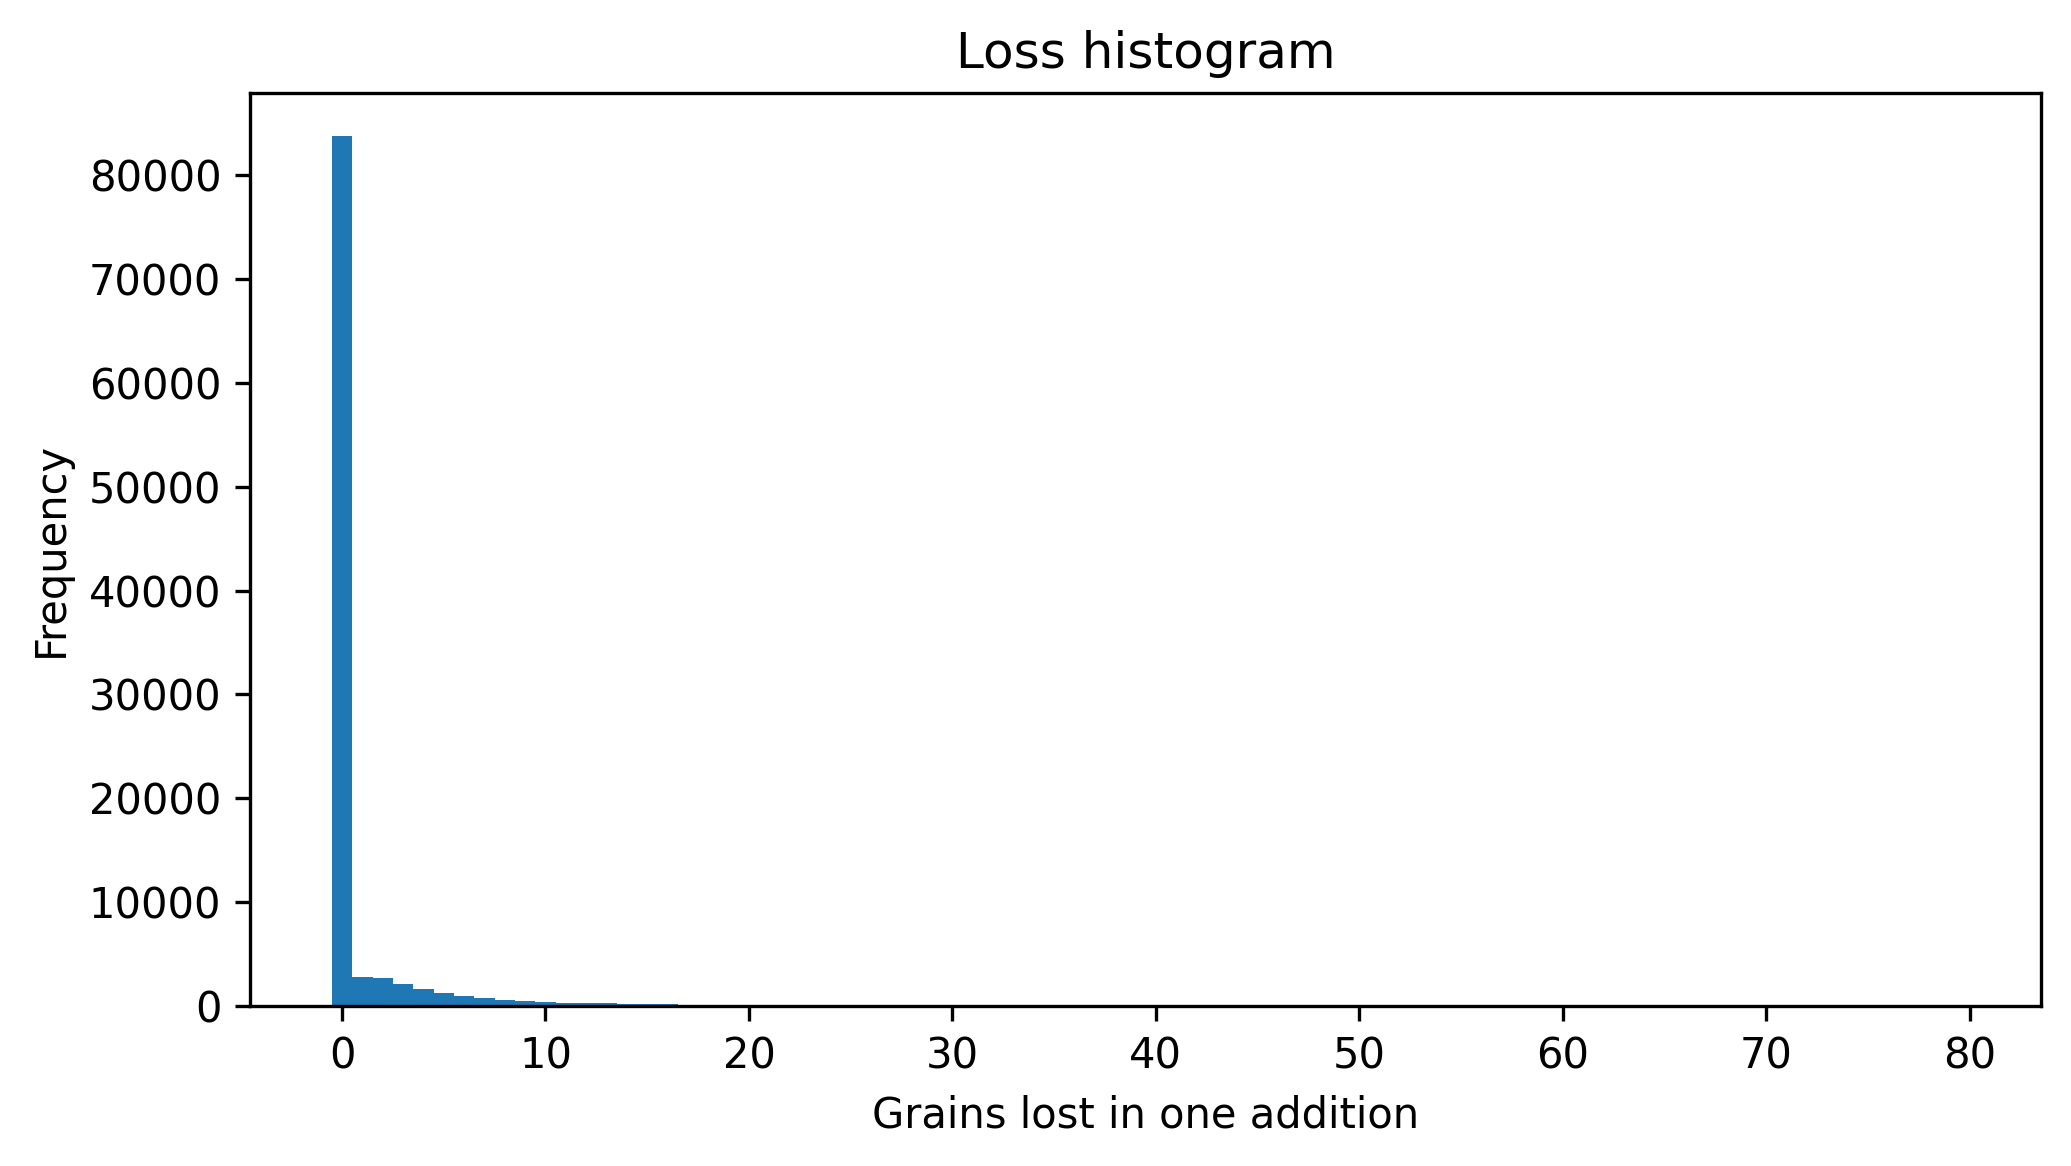
\includegraphics[width=0.45\textwidth]{figures/loss_histogram.png}
    \hfill
    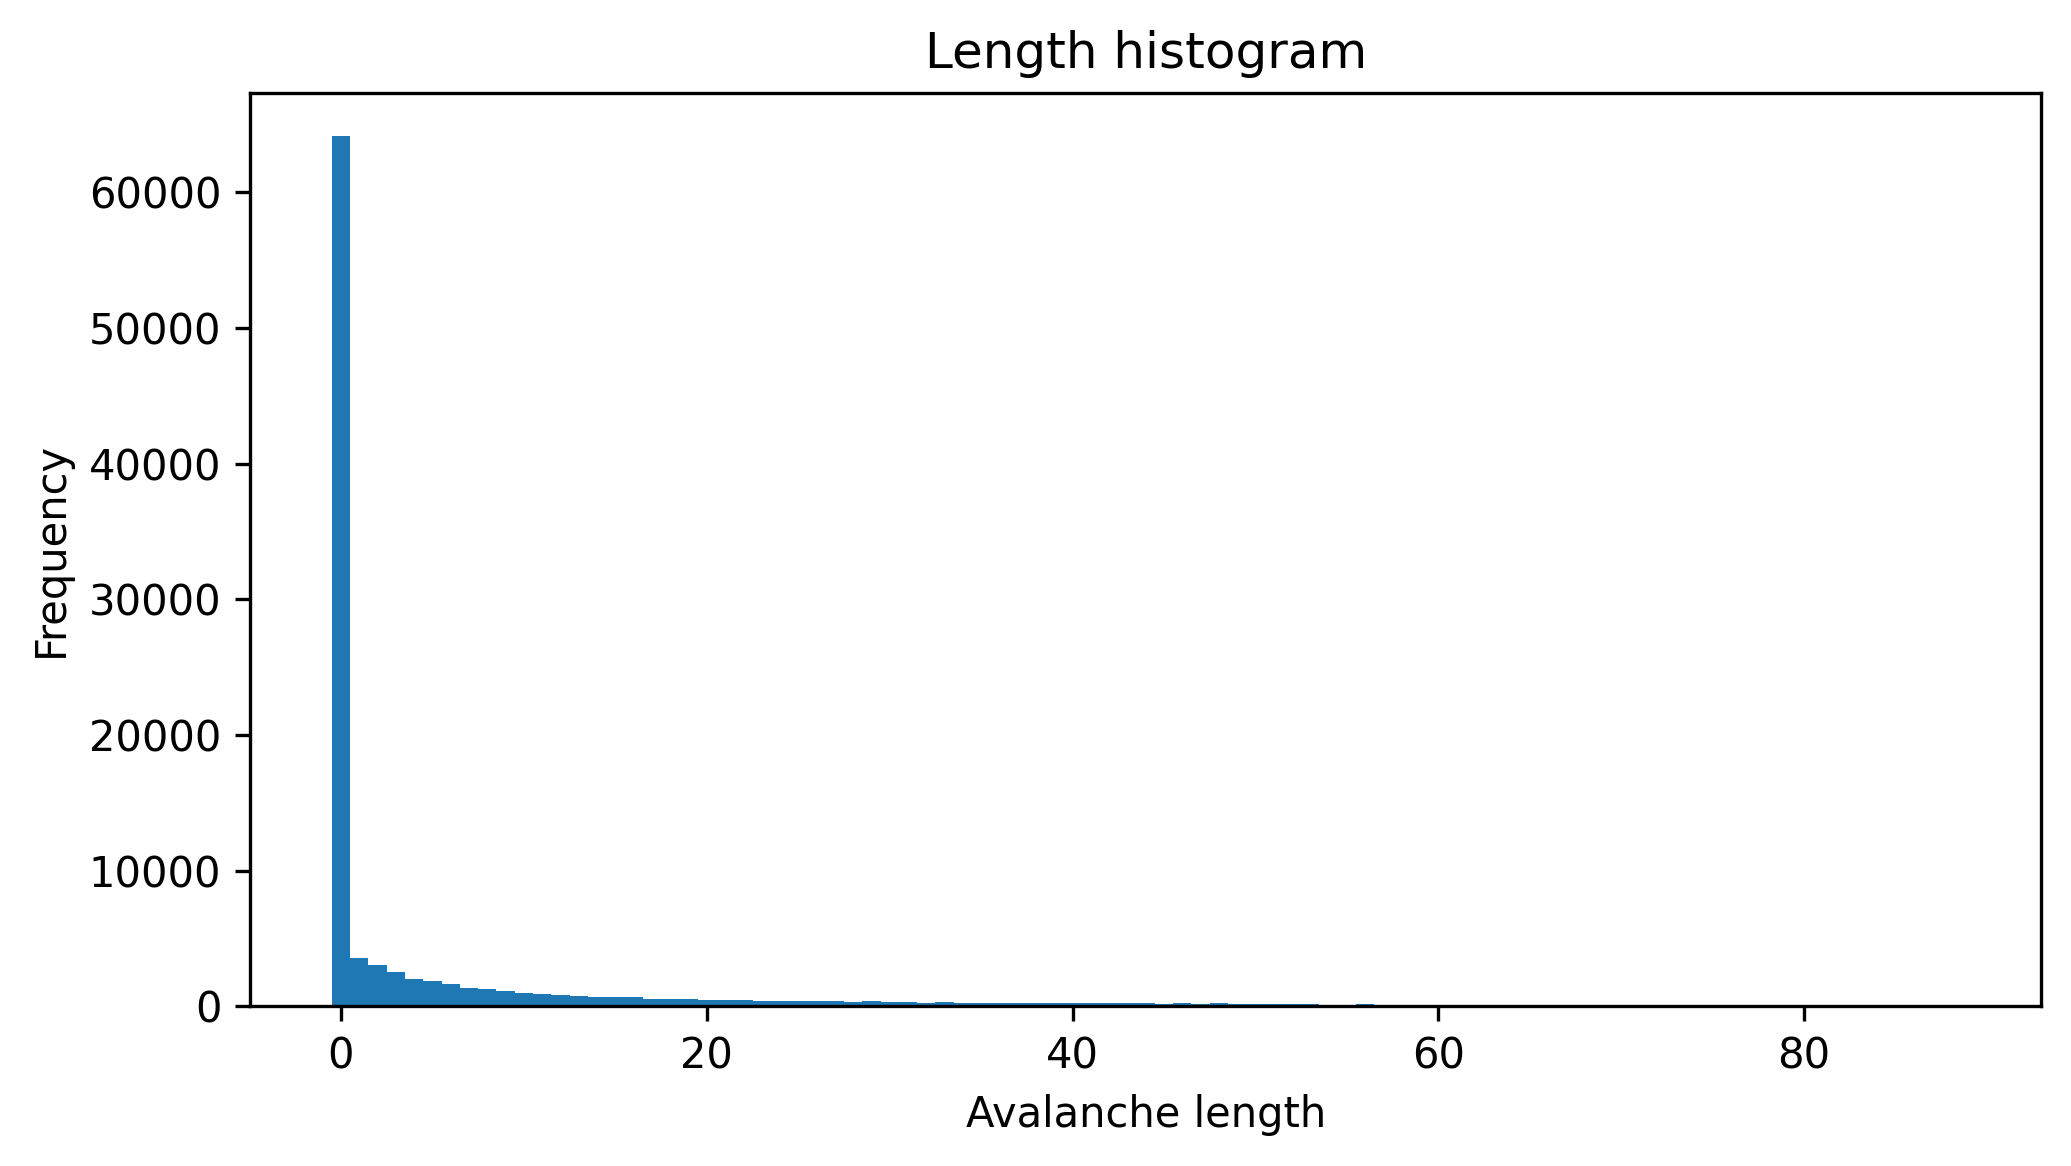
\includegraphics[width=0.45\textwidth]{figures/length_histogram.png}

    \caption{Histograms of avalanche topples, area, loss and length. The distributions are
    strongly right-skewed, with many small avalanches and relatively few large avalanches.}
    \label{fig:q7_histograms}
\end{figure}

\subsection{Log--log Plots and Power-law Behaviour}

To test whether the distributions are approximately power-law distributed, I plotted the
frequency data on log--log axes. A power-law distribution has the form
\[
P(x) \sim Cx^{-\alpha},
\]
where \(x\) is the avalanche observable and \(\alpha\) is the power-law exponent. Taking
logarithms gives
\[
\log P(x) = \log C - \alpha \log x.
\]
Therefore, if the distribution follows a power law, the log--log plot should be approximately
linear, with slope \(-\alpha\).

The log--log plots are shown in Figure~\ref{fig:q7_loglog}. The plots for topples and area
show the clearest approximately linear regions, suggesting that these two quantities are
approximately power-law distributed over an intermediate range. This is consistent with
self-organized criticality: there is no single characteristic avalanche size, and avalanches
occur over a wide range of scales.

\begin{figure}[htbp]
    \centering

    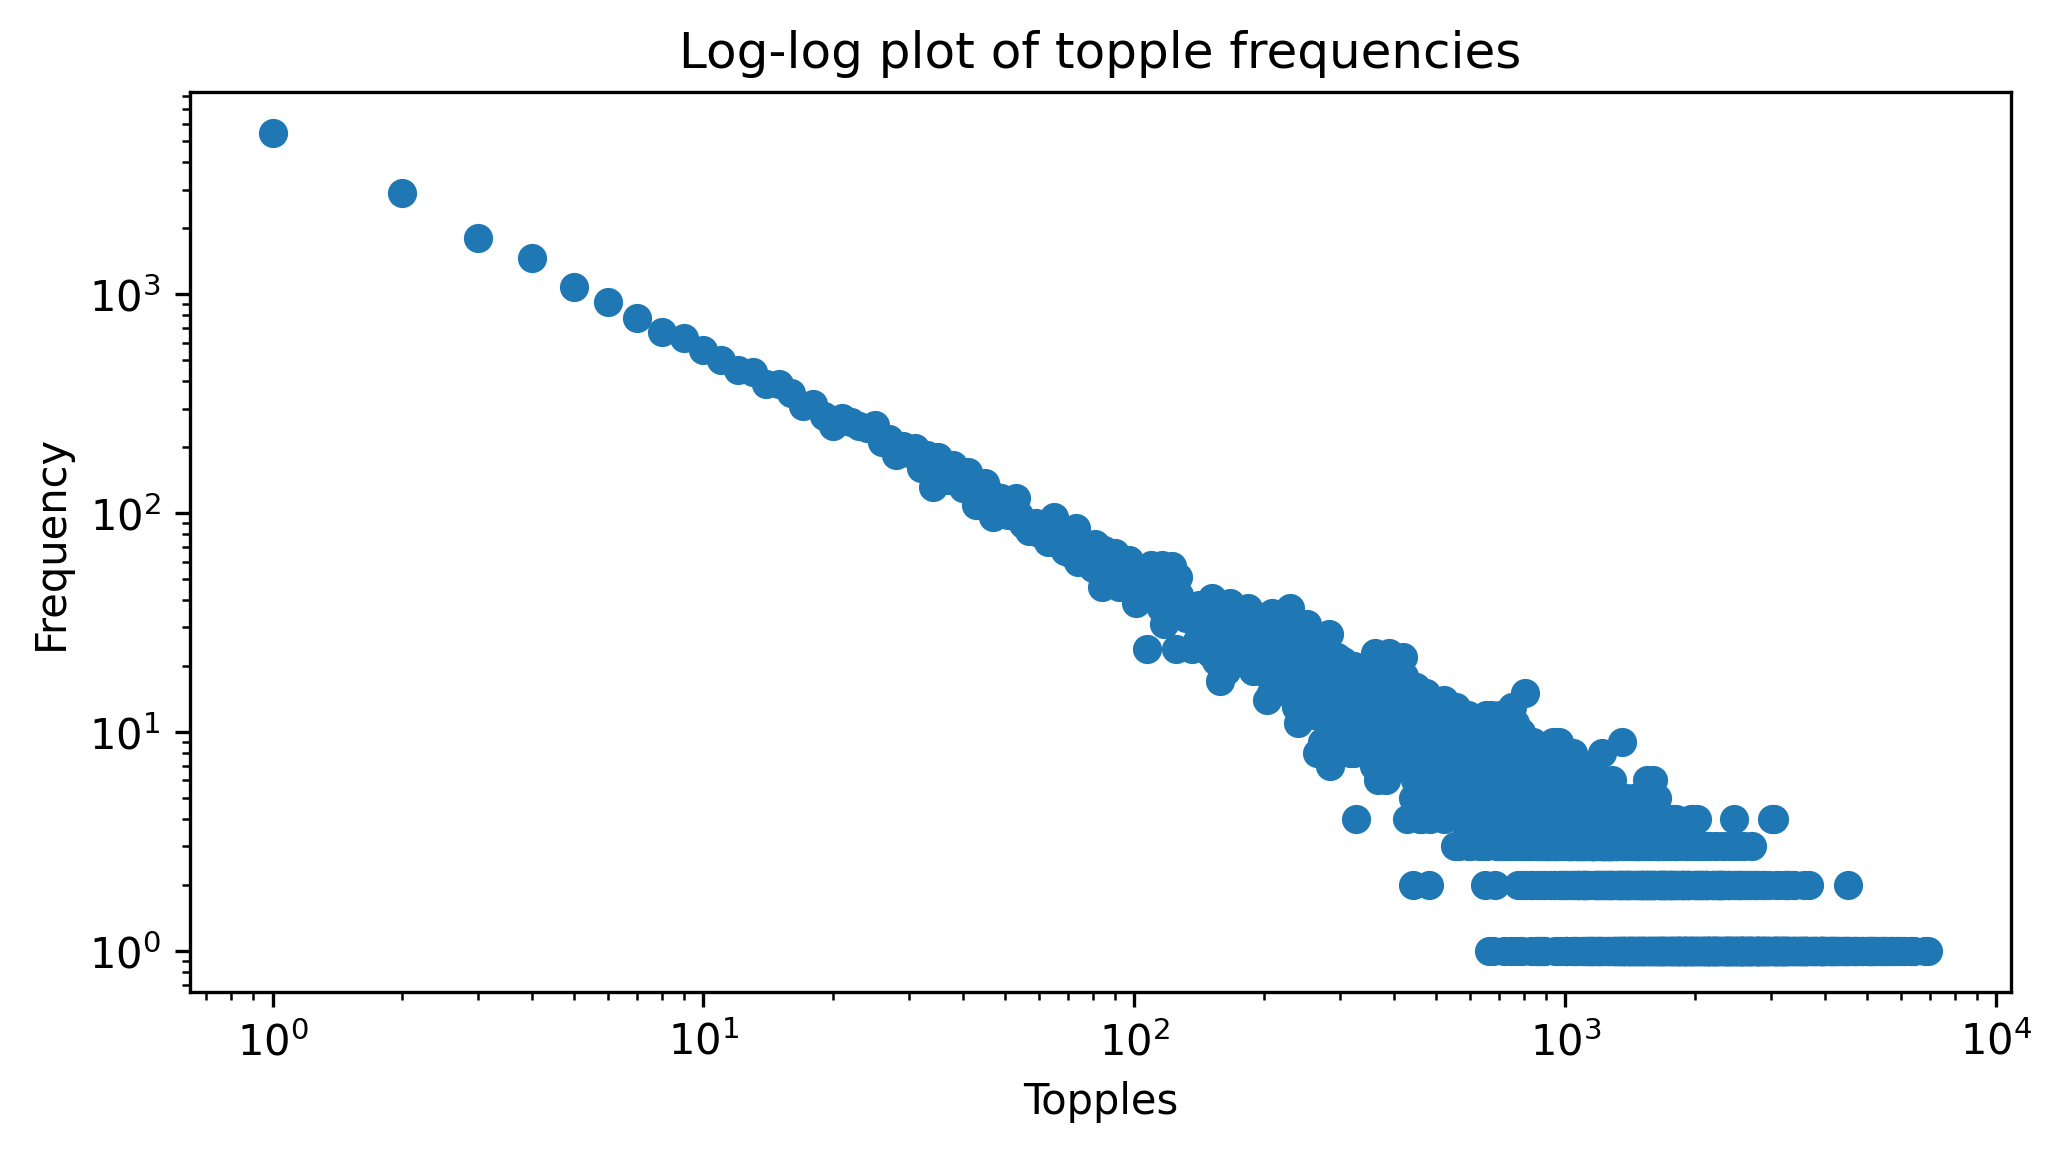
\includegraphics[width=0.45\textwidth]{figures/topple_loglog.png}
    \hfill
    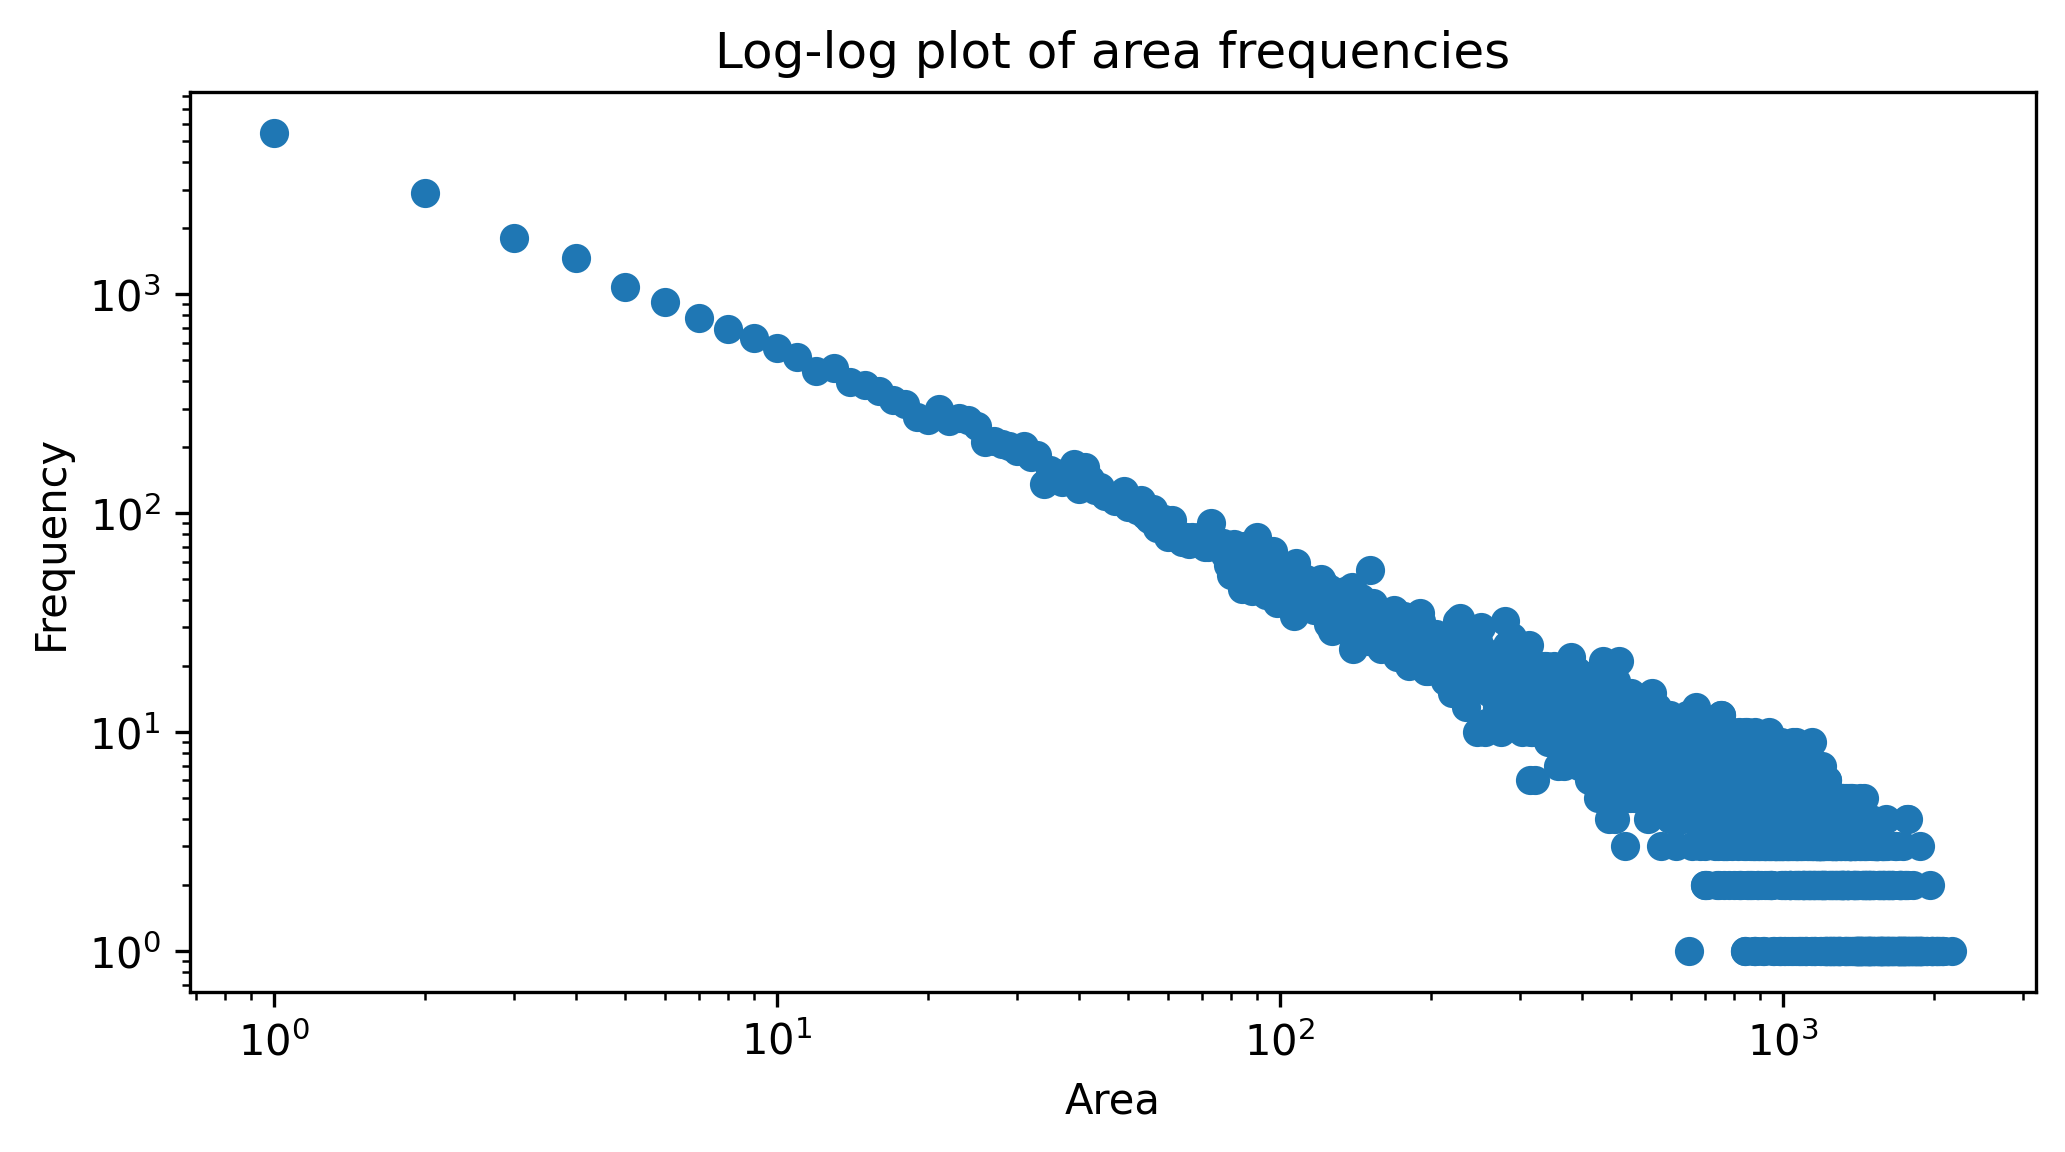
\includegraphics[width=0.45\textwidth]{figures/area_loglog.png}

    \vspace{0.4cm}

    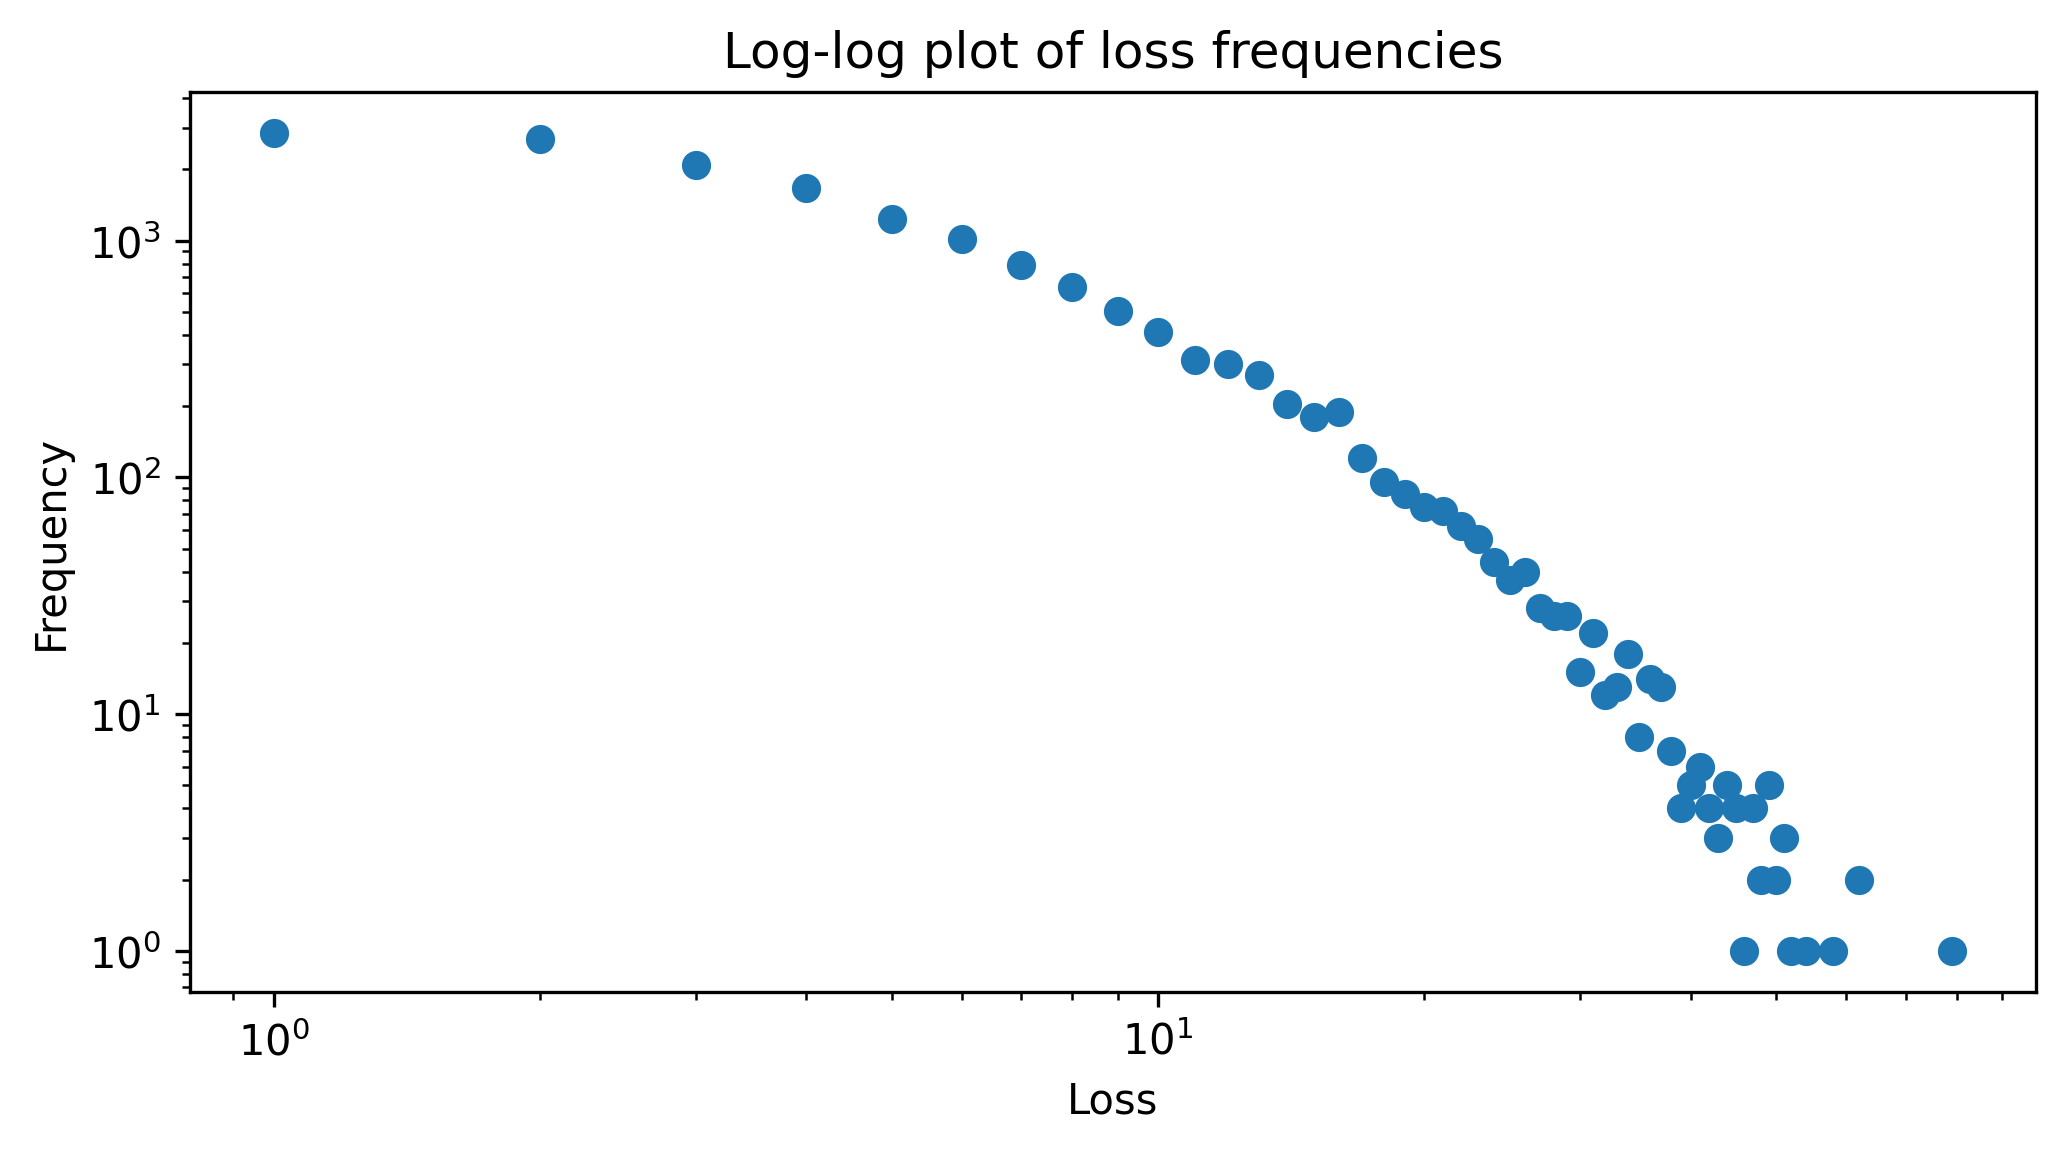
\includegraphics[width=0.45\textwidth]{figures/loss_loglog.png}
    \hfill
    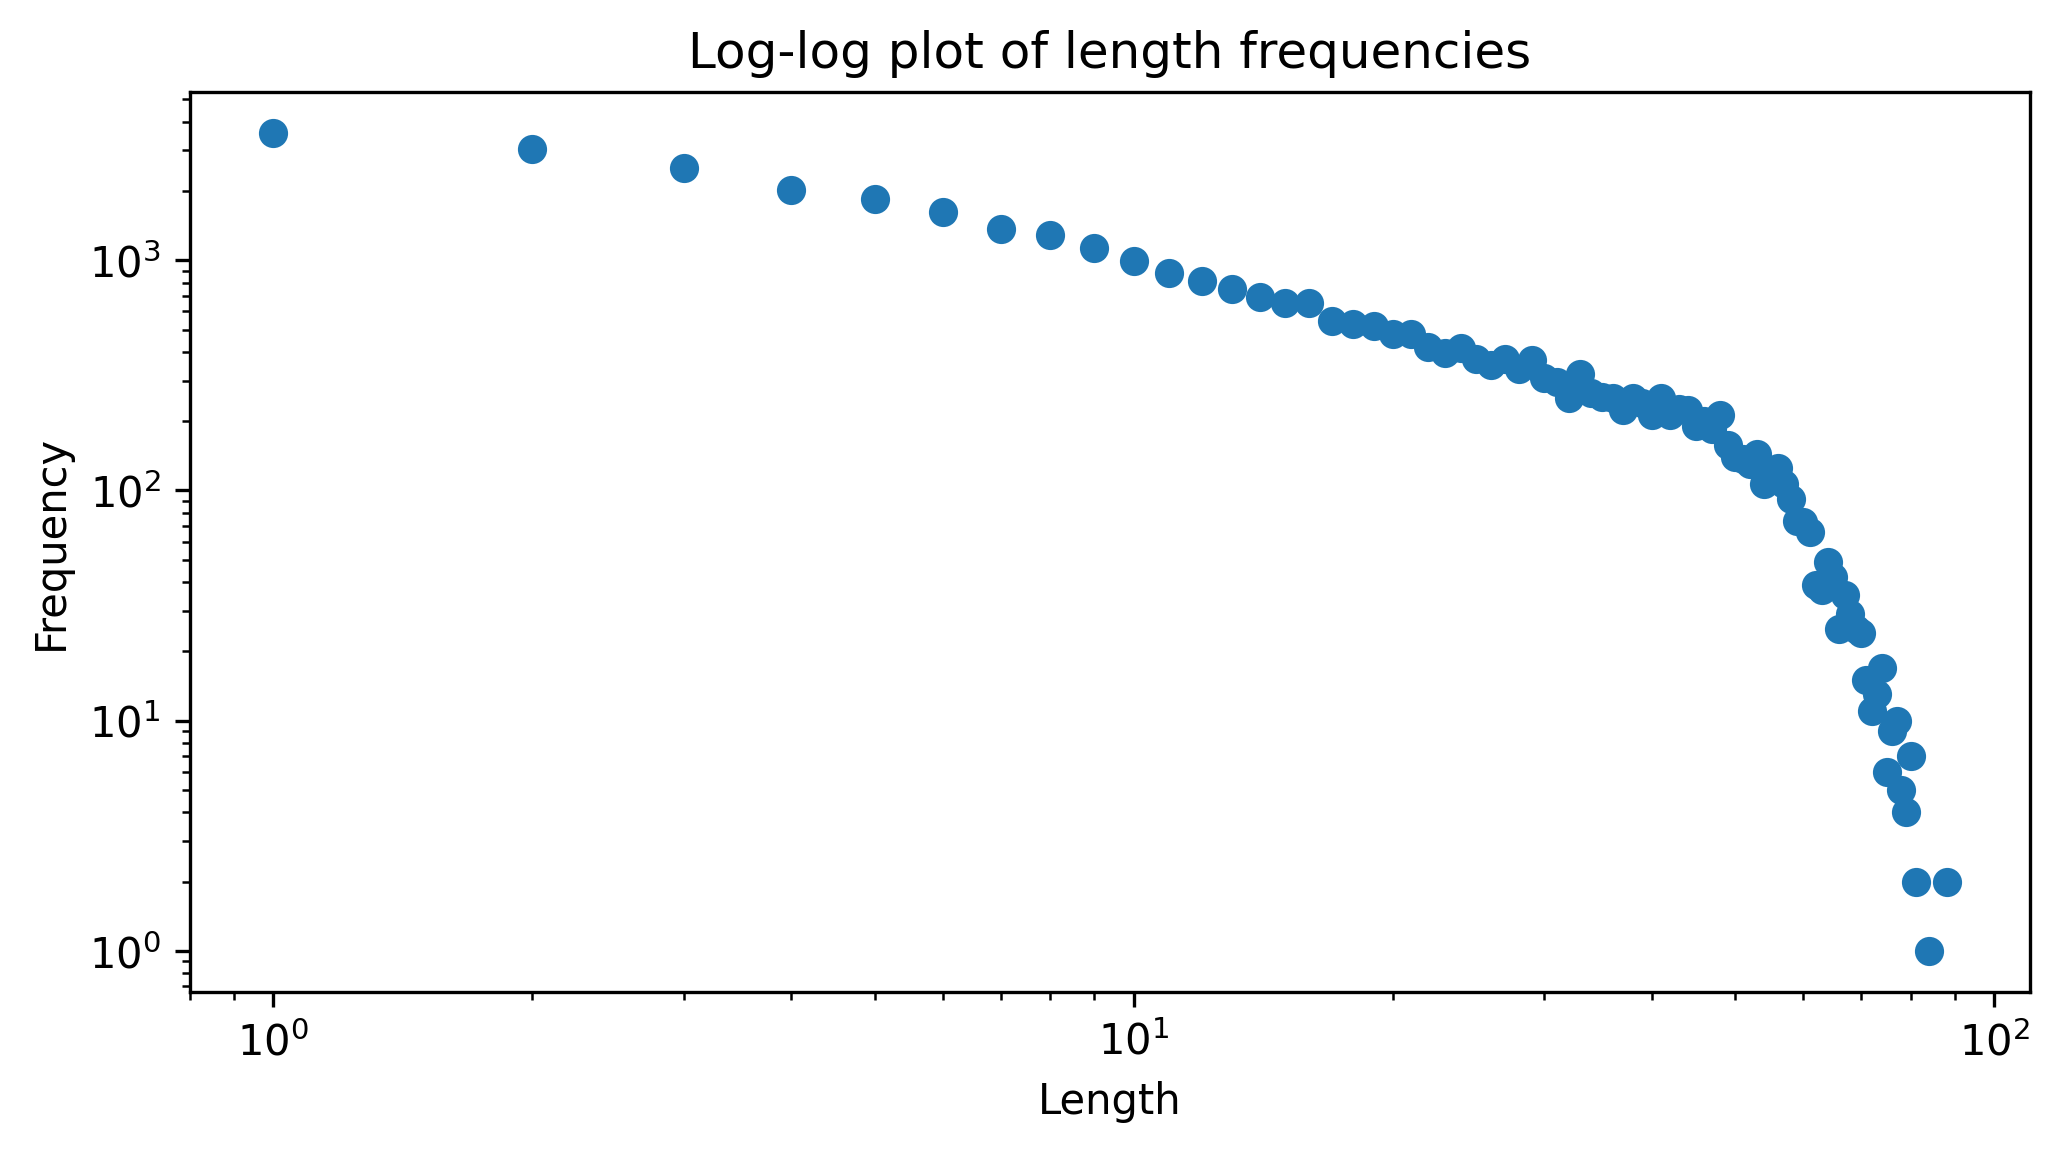
\includegraphics[width=0.45\textwidth]{figures/length_loglog.png}

    \caption{Log--log plots of the avalanche distributions. Approximately linear behaviour
    in the intermediate region suggests power-law behaviour, especially for topples and area.}
    \label{fig:q7_loglog}
\end{figure}

The distributions are not perfect power laws across the whole range. For very small
avalanches, discreteness effects are important because the observables take small integer
values. For very large avalanches, the finite lattice size imposes a cutoff, since an avalanche
cannot spread beyond the boundary of the grid. Thus the power-law behaviour is expected
only in an intermediate scaling region.

The loss distribution is less clean than the distributions for topples and area. This is because
many avalanches do not reach the boundary, so they lose no grains. Positive loss only occurs
when an avalanche reaches the edge of the lattice. Therefore, the loss distribution is more
strongly affected by the boundary condition and the finite size of the system.

The length distribution is also heavy-tailed, but it has a clear finite-size cutoff. This is
expected because the maximum possible avalanche length is limited by the dimensions of
the lattice. Hence the length distribution may only show approximate power-law behaviour
over a restricted intermediate range.

\subsection{Estimated Form of the Distributions}

The results may be summarised as follows:

\begin{table}[htbp]
    \centering
    \begin{tabular}{c|c|p{0.45\textwidth}}
        \hline
        Quantity & Observed distribution & Comment \\
        \hline
        Topples & Approximate power law & The log--log plot has a clear decreasing approximately linear region. \\
        Area & Approximate power law & Similar to topples, with strong evidence of scale-free behaviour. \\
        Loss & Heavy-tailed, less clean & Strongly affected by boundary loss and many zero-loss avalanches. \\
        Length & Heavy-tailed with cutoff & Limited by the finite size of the lattice. \\
        \hline
    \end{tabular}
    \caption{Summary of the avalanche distributions observed in the simulation.}
    \label{tab:q7_distribution_summary}
\end{table}

If a straight-line fit is applied to the approximately linear region of each log--log plot, then
the power-law exponent can be estimated from the fitted slope. If the fitted line is
\[
\log P(x) = a + b \log x,
\]
then
\[
\alpha = -b.
\]
Only the intermediate region should be used for this fit, because the small-avalanche region
is affected by discreteness and the large-avalanche region is affected by finite-size cutoff.

Overall, the avalanche statistics provide evidence that the BTW sandpile model exhibits
self-organized criticality. The model produces many small avalanches and a few large
avalanches, with approximately power-law behaviour in the avalanche observables. This
indicates scale invariance and shows that the system does not have a characteristic
avalanche size.

It remains to find a fit for the exponent.

\section{Abelian Property of the BTW Model}
\label{sec:abelian_property}

The Bak--Tang--Wiesenfeld model has an important mathematical property: the order of
topplings does not affect the final stable configuration. This is called the \textbf{Abelian
property}. To describe this more carefully, we introduce the toppling matrix and toppling
operator.

Let \(\Lambda\) be a finite subset of \(\mathbb{Z}^d\), representing the lattice. In this project,
we mainly consider the two-dimensional case \(d=2\). A sandpile configuration is a function
\[
h : \Lambda \to \mathbb{N}_0,
\]
where \(h(x)\) is the number of grains of sand at the lattice site \(x \in \Lambda\).

A configuration is called \textbf{stable} if
\[
h(x) < z_c
\qquad
\text{for all } x \in \Lambda,
\]
where \(z_c\) is the stability threshold. A configuration is \textbf{unstable} if there exists at
least one site \(x \in \Lambda\) such that
\[
h(x) \geq z_c.
\]

For the two-dimensional BTW model, the threshold is
\[
z_c = 4,
\]
because a site topples when it has four or more grains.

\subsection{Question 9: Conditions on the Toppling Matrix}

The toppling matrix \(\Delta(x,y)\) describes how sand is redistributed when the site \(x\)
topples. The project gives the following conditions:
\[
\forall x,y \in \Lambda,\ x \neq y, 
\qquad
\Delta(x,y)=\Delta(y,x) \geq 0,
\tag{4a}
\]
\[
\forall x \in \Lambda,
\qquad
\Delta(x,x)<0,
\tag{4b}
\]
\[
\forall x \in \Lambda,
\qquad
\sum_{y \in \Lambda} \Delta(x,y) \leq 0,
\tag{4c}
\]
and
\[
\sum_{x,y \in \Lambda} \Delta(x,y) < 0.
\tag{4d}
\]

Condition \((4a)\) says that, for two different sites \(x\) and \(y\), the amount of sand
transferred between neighbouring sites is non-negative and symmetric. The non-negativity
is natural because a toppling should add grains to neighbouring sites, not remove grains
from them. The symmetry condition means that the interaction between sites is undirected:
if \(x\) is a neighbour of \(y\), then \(y\) is also a neighbour of \(x\).

Condition \((4b)\) says that
\[
\Delta(x,x)<0.
\]
This means that when site \(x\) topples, it loses grains. This is necessary because toppling
is supposed to reduce the height of an unstable site. In the two-dimensional BTW model,
the toppled site loses four grains, so \(\Delta(x,x)=-4\).

Condition \((4c)\) says that the total change in the amount of sand caused by toppling one
site is less than or equal to zero:
\[
\sum_{y \in \Lambda} \Delta(x,y) \leq 0.
\]
This means that a toppling cannot create sand overall. In the interior of the lattice, the sum
is equal to zero because the four grains lost by \(x\) are transferred to its four neighbours.
At the boundary, some grains may leave the lattice, so the sum is negative.

Condition \((4d)\) says that
\[
\sum_{x,y \in \Lambda} \Delta(x,y) < 0.
\]
This ensures that the system is dissipative overall. In other words, somewhere in the lattice
there must be a possibility for sand to leave the system. This is important for the model to
reach a statistically stationary state. Without dissipation, sand would keep accumulating
and the system would not stabilize in the same way.

\subsection{Question 10: The BTW Toppling Matrix}

In the BTW model, the toppling matrix is defined by
\[
\Delta(x,y)
=
\begin{cases}
-2d, & x=y, \\
1, & x \text{ and } y \text{ are nearest neighbours}, \\
0, & \text{otherwise}.
\end{cases}
\]
In the two-dimensional case, \(d=2\), so this becomes
\[
\Delta(x,y)
=
\begin{cases}
-4, & x=y, \\
1, & x \text{ and } y \text{ are nearest neighbours}, \\
0, & \text{otherwise}.
\end{cases}
\]

This definition exactly represents the BTW toppling rule. When a site \(x\) topples, it loses
four grains:
\[
h(x) \mapsto h(x)-4.
\]
Each of its four nearest neighbours receives one grain:
\[
h(y) \mapsto h(y)+1
\]
whenever \(y\) is a nearest neighbour of \(x\).

We now verify that this matrix satisfies the four conditions.

First, if \(x \neq y\), then
\[
\Delta(x,y)=1
\]
when \(x\) and \(y\) are nearest neighbours, and otherwise
\[
\Delta(x,y)=0.
\]
Thus
\[
\Delta(x,y) \geq 0.
\]
Also, the nearest-neighbour relation is symmetric, so
\[
\Delta(x,y)=\Delta(y,x).
\]
Therefore condition \((4a)\) is satisfied.

Second, for every site \(x\),
\[
\Delta(x,x)=-4<0.
\]
Therefore condition \((4b)\) is satisfied.

Third, consider the row sum
\[
\sum_{y \in \Lambda} \Delta(x,y).
\]
If \(x\) is an interior site, then it has four nearest neighbours inside the lattice. Hence
\[
\sum_{y \in \Lambda} \Delta(x,y)
=
-4+1+1+1+1
=
0.
\]
If \(x\) is a boundary site, then it has fewer than four neighbours inside the lattice. For
example, an edge site has three neighbours and a corner site has two neighbours. Therefore
the row sum is negative:
\[
-4+3=-1
\]
for an edge site, and
\[
-4+2=-2
\]
for a corner site. Hence, in all cases,
\[
\sum_{y \in \Lambda} \Delta(x,y) \leq 0.
\]
So condition \((4c)\) is satisfied.

Finally, because the lattice has boundary sites, there are sites for which the row sum is
strictly negative. Therefore,
\[
\sum_{x,y \in \Lambda} \Delta(x,y) < 0.
\]
This verifies condition \((4d)\). The strict negativity comes from grains being lost when
boundary sites topple.

Thus the BTW toppling matrix satisfies all the required conditions. The stability threshold
in the two-dimensional BTW model is
\[
z_c=4.
\]

\subsection{Question 11: Commutativity of Toppling Operators}

Using the toppling matrix, we define the toppling operator \(T_x\). If \(x\) is unstable, then
toppling at \(x\) maps a configuration \(h\) to a new configuration \(T_x h\), where
\[
(T_xh)(y)
=
h(y)+\Delta(x,y).
\]
In other words, toppling at \(x\) adds the row \(\Delta(x,\cdot)\) of the toppling matrix to
the height configuration.

More explicitly, in the two-dimensional BTW model,
\[
(T_xh)(x)=h(x)-4,
\]
and if \(y\) is a nearest neighbour of \(x\), then
\[
(T_xh)(y)=h(y)+1.
\]
All other sites are unchanged.

Now suppose that \(x\) and \(x'\) are both unstable sites in the configuration \(h\). We want
to show that the toppling operators commute:
\[
T_xT_{x'}h = T_{x'}T_xh.
\]

For any site \(y \in \Lambda\), first topple \(x'\), then topple \(x\). We get
\[
(T_xT_{x'}h)(y)
=
(T_{x'}h)(y)+\Delta(x,y).
\]
Since
\[
(T_{x'}h)(y)=h(y)+\Delta(x',y),
\]
we have
\[
(T_xT_{x'}h)(y)
=
h(y)+\Delta(x',y)+\Delta(x,y).
\]

On the other hand, if we first topple \(x\), then topple \(x'\), we get
\[
(T_{x'}T_xh)(y)
=
(T_xh)(y)+\Delta(x',y).
\]
Since
\[
(T_xh)(y)=h(y)+\Delta(x,y),
\]
we have
\[
(T_{x'}T_xh)(y)
=
h(y)+\Delta(x,y)+\Delta(x',y).
\]

But addition of integers is commutative, so
\[
h(y)+\Delta(x',y)+\Delta(x,y)
=
h(y)+\Delta(x,y)+\Delta(x',y).
\]
Therefore, for every site \(y \in \Lambda\),
\[
(T_xT_{x'}h)(y)
=
(T_{x'}T_xh)(y).
\]
Hence
\[
T_xT_{x'}h = T_{x'}T_xh.
\]

This proves that toppling operators commute when both topplings are allowed. Therefore,
the order in which unstable sites are toppled does not affect the resulting configuration.
This proves the Abelian property of the BTW sandpile model. Consequently, in the numerical implementation, we do not need to keep track of a unique physically meaningful order of topplings. Instead, all currently unstable sites can be stored in a queue and processed one by one. Although the queue imposes some computational order, the Abelian property guarantees that the final stable configuration is independent of this chosen order.